\documentclass[border=10pt]{standalone}
\usepackage{tikz}
\usetikzlibrary{arrows.meta, shapes, calc}

\begin{document}

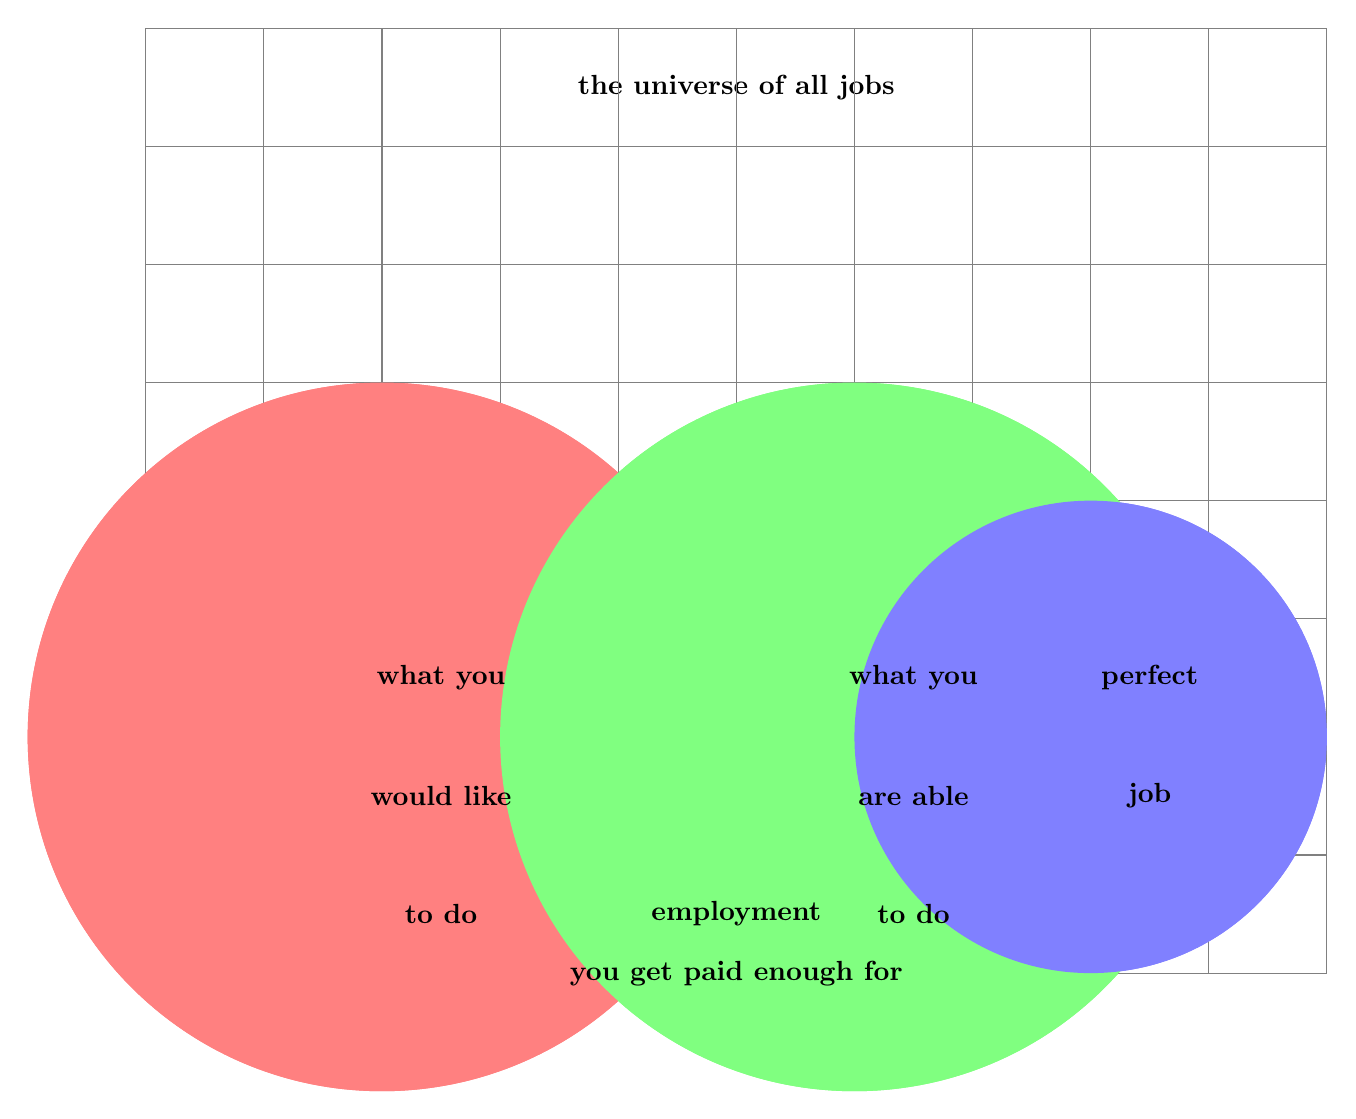
\begin{tikzpicture}[scale=1.5]
    % Background
    \fill[white] (0,0) rectangle (10,8);
    
    % Title
    \node at (5,7.5) {\textbf{the universe of all jobs}};
    
    % Venn Diagram
    \fill[red!50] (2,2) circle (3);
    \fill[green!50] (6,2) circle (3);
    \fill[blue!50] (8,2) circle (2);
    \fill[blue!50] (8,2) circle (1);
    \fill[blue!50] (8,2) circle (0.5);
    \fill[blue!50] (8,2) circle (0.25);
    
    % Labels
    \node at (2.5,2.5) {\textbf{what you}};
    \node at (2.5,1.5) {\textbf{would like}};
    \node at (2.5,0.5) {\textbf{to do}};
    
    \node at (6.5,2.5) {\textbf{what you}};
    \node at (6.5,1.5) {\textbf{are able}};
    \node at (6.5,0.5) {\textbf{to do}};
    
    \node at (8.5,2.5) {\textbf{perfect}};
    \node at (8.5,1.5) {\textbf{job}};
    
    \node at (5,0.5) {\textbf{employment}};
    \node at (5,0) {\textbf{you get paid enough for}};
    
    % Grid
    \draw[gray, thin] (0,0) grid (10,8);
    
    % Lines
    \draw[red, thick] (2,2) -- (6,2);
    \draw[red, thick] (6,2) -- (8,2);
    \draw[red, thick] (8,2) -- (8,2);
    \draw[red, thick] (8,2) -- (8,2);
    \draw[red, thick] (8,2) -- (8,2);
    
    % Subplots
    \fill[red!50] (2,2) circle (3);
    \fill[green!50] (6,2) circle (3);
    \fill[blue!50] (8,2) circle (2);
    \fill[blue!50] (8,2) circle (1);
    \fill[blue!50] (8,2) circle (0.5);
    \fill[blue!50] (8,2) circle (0.25);
    
    % Text in subplots
    \node at (2.5,2.5) {\textbf{what you}};
    \node at (2.5,1.5) {\textbf{would like}};
    \node at (2.5,0.5) {\textbf{to do}};
    
    \node at (6.5,2.5) {\textbf{what you}};
    \node at (6.5,1.5) {\textbf{are able}};
    \node at (6.5,0.5) {\textbf{to do}};
    
    \node at (8.5,2.5) {\textbf{perfect}};
    \node at (8.5,1.5) {\textbf{job}};
    
    \node at (5,0.5) {\textbf{employment}};
    \node at (5,0) {\textbf{you get paid enough for}};
    
\end{tikzpicture}

\end{document}